\documentclass[sigconf,nonacm]{aamas}
\usepackage{amsmath,amssymb,booktabs,balance}
\setcopyright{none}
\settopmatter{printacmref=false,printfolios=true}
\acmConference[Research manuscript]{Research manuscript}{September 2026}{}{}
\acmYear{2026}
\acmDOI{}
\acmISBN{}
\title[Private Participation in Agent Contract Selection]{Private Participation in Agent Contract Selection:\texorpdfstring{\\}{ }Exact Frontiers and Incompatible Optima}
\author{Shivam Gupta}
\affiliation{\institution{Independent Researcher}\city{Delhi}\country{India}}
\email{shivam1720406@gmail.com}
\keywords{Private participation, differential privacy, agent contracts}
\newcommand{\E}{\mathcal E}
\newcommand{\F}{\mathcal F}
\newcommand{\PP}{\mathcal P}
\newcommand{\botout}{\bot}
\newcommand{\ind}{\mathbf 1}
\newtheorem{theorem}{Theorem}
\newtheorem{proposition}[theorem]{Proposition}
\newtheorem{corollary}[theorem]{Corollary}
\begin{abstract}
An agent may hide its participation decision in messages while revealing it through an executed agreement. We study a trusted broker that selects at most one public contract, each requiring a specified set of agents with private participation bits. Contracts must be feasible, and the executed identifier or abstention is public. We characterize exactly the distributions attainable at any fixed participation profile under $(\epsilon,\delta)$-differential privacy: they form a fractional packing polytope whose participant capacities are $\delta$. A fixed contract lottery followed by a private veto extends every point of this polytope to a mechanism private on the entire profile space. Consequently, every pointwise utility optimum is independent of $\epsilon$. These optima need not be jointly attainable. For five bilateral contracts arranged in a cycle, we derive the exact Pareto frontier between full-participation success and average success after one withdrawal under $(0,\delta)$-privacy. An explicit $(\log 2,\delta)$-private mechanism raises optimal withdrawal success from $7\delta/4$ to $2\delta$, despite unchanged pointwise bounds. Computation verifies 762 small-menu comparisons, 381 rational primal--dual certificates, 66 rational mechanisms, and 288 six-agent policy comparisons. The results give an auditable design test for private agent contracting and isolate a distinction between local attainability and compatible adaptation.
\end{abstract}
\begin{document}
\maketitle
\hypersetup{pdfauthor={Shivam Gupta}}

\section{Introduction}
Consider a broker choosing among candidate service agreements. One agreement requires a supplier and a logistics agent; another requires a different supplier and an inspection agent. Each agent privately reports whether it can participate in the current session. A completed agreement publicly identifies its required parties. Even if the broker hides all reports and negotiation messages, executing an agreement certifies that those parties were available. This information may expose an organization's operating capacity or willingness to enter a particular market.

There are two distinct design questions. First, how often can a broker execute an agreement without violating participation privacy or involving an unavailable agent? Second, can a broker attain that maximum at every participation profile by adapting its selection policy? Treating these as the same question overlooks constraints that relate the distributions at neighboring profiles.

Privacy limits on useful allocations are established in matching, exchange, and constrained optimization~\cite{hsu2016,kannan2018,munoz2021}. The present work does not claim that outcome leakage, randomized selection, or the conflict between privacy and hard feasibility is new. We study the exact structure of that conflict for a public contract menu and binary participation. This deliberately narrow model admits both a complete local characterization and a small example with a sharp global tradeoff.

Our first result describes the entire set of achievable output distributions at an arbitrary profile. Let $p_e$ be the probability of selecting contract $e$. Every agent $i$ imposes the capacity constraint
\begin{equation}\label{eq:load-intro}
\sum_{e\ni i}p_e\leq\delta.
\end{equation}
This follows by comparing the profile to one in which $i$ withdraws: the event that an executed contract requires $i$ has probability zero in the latter. Together with normalization and feasibility, these constraints are sufficient. A public lottery with probabilities $p_e$, followed by a private veto, realizes the desired row and remains private at every other profile. The resulting optimization is a standard fractional packing problem; the contribution is its exact identification with an attainable-mechanism projection.

The second result shows why this characterization is not an adaptive algorithm. On a five-cycle of bilateral contracts, the optimal full-participation row and an optimal one-withdrawal row assign incompatible probabilities to a particular event. We derive the complete nondominated tradeoff at $\epsilon=0$, construct both endpoints, and show that increasing $\epsilon$ can improve a public-prior objective even though it changes none of the individual profile optima. Thus privacy can limit the compatibility of individually attainable decisions, beyond limiting each decision in isolation.

The artifact, named \emph{Consent Lottery}, contains a packing optimizer, an exact rational sampler, a full-profile privacy LP, four reproducible figures, and separate result-verification scripts. Evaluation combines exact finite calculations with synthetic contract menus. It establishes the stated mechanism properties, rather than improved language-model bargaining performance. A broker can use the result to test whether a success target is compatible with its chosen privacy guarantee.

\begin{figure*}[t]
\centering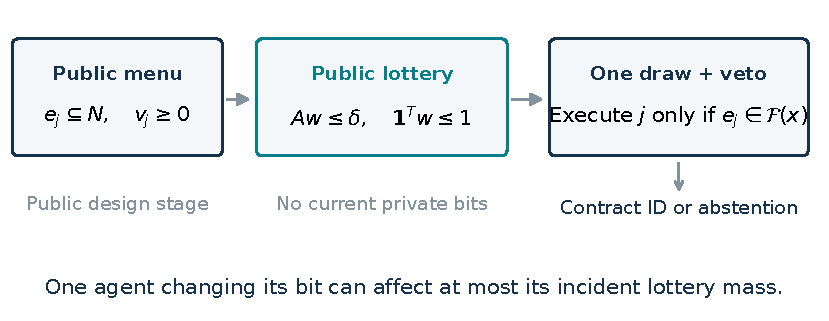
\includegraphics[width=.94\textwidth]{figures/01-lottery.pdf}
\caption{Consent Lottery separates public mechanism design from the private participation check. A veto produces abstention and consumes the draw. Renormalizing over the privately feasible menu implements a different mechanism. The guarantee concerns the released outcome; the broker is trusted.}
\Description{A public contract menu feeds a constrained public lottery, followed by a single draw and a private feasibility veto.}
\label{fig:pipeline}
\end{figure*}

\section{Related Work}
\paragraph{Private allocation and hard feasibility.}
Hsu et al.~\cite{hsu2016} study matching and allocation under joint differential privacy, which excludes an agent's own allocation from the view protected against that agent's data. Kannan et al.~\cite{kannan2018} establish limits on private, individually rational exchange and introduce a weaker marginal guarantee. We instead protect binary participation against an observer of the public executed contract. The exclusion event behind \eqref{eq:load-intro} is an instance of the established support obstruction. Our addition is an exact, menu-dependent attainable-row polytope and its globally feasible extension.

Mu\~noz Medina et al.~\cite{munoz2021} develop private optimization with linear constraints that must always hold. They perturb private bounds in linear constraints and analyze the resulting optimization error. Damle et al.~\cite{damle2021} randomize multi-agent constraint optimization and explicitly distinguish their soft-constraint setting from hard-constraint leakage. We release a discrete contract identifier and require every named agent to participate. The characterization uses neither noisy estimates of constraints nor soft penalties.

\paragraph{Optimal mechanisms.}
Finite privacy mechanisms admit established LP formulations~\cite{ghosh2012}. Universal optimality and its failure have also been studied extensively~\cite{brenner2010,fernandes2022}. In particular, Brenner and Nissim use cycles in a \emph{query-output privacy graph} to prove nonexistence results. Our five-cycle is instead a \emph{contract-incidence graph}: the privacy graph remains the five-dimensional Boolean cube. We do not claim a new general impossibility of universal optimality. We study approximate privacy with hard output exclusions. We derive an exact frontier for two objectives and specify mechanisms on all 32 inputs. Binary mechanisms based on boundary conditions~\cite{torkamani2023} have a different output structure: retaining the executed contract's identity makes multi-output events essential here.

\paragraph{Agent contracts and negotiation privacy.}
Recent work studies enforceable contracts between language-model agents~\cite{wyse2026} and privacy for the behavioral traces of negotiation~\cite{rani2026}. Our analysis concerns a broker's terminal output and is independent of the language model producing candidate agreements. It neither replicates those systems nor evaluates their reported performance. An LLM may help construct a public menu, but if construction itself depends on protected participation bits, it is an additional private release outside our guarantee.

\section{Model and Evaluation Targets}\label{sec:model}
There are $n$ agents, $N=\{1,\ldots,n\}$, and a public finite set $\E$ of $m$ nonempty contracts. A contract $e\subseteq N$ specifies its required agents. Each has a nonnegative public utility $v_e$; unit utility measures agreement probability. Private input $x\in\{0,1\}^n$ records participation. Write
\[
\F(x)=\{e\in\E:x_i=1\text{ for every }i\in e\}.
\]
A randomized broker $M$ outputs $e\in\E$ or abstention $\botout$. Its row is $P_x(o)=\Pr[M(x)=o]$. \emph{Hard feasibility} requires $P_x(e)=0$ whenever $e\notin\F(x)$. At most one contract executes. This is not a simultaneous matching problem: two contracts may overlap, but they cannot both be selected in one output.

Profiles $x\sim_i y$ differ only in bit $i$. For $\epsilon\geq0$ and participant budgets $\boldsymbol\delta\in[0,1]^n$, privacy requires, for every output event $S$,
\begin{equation}\label{eq:dp}
 P_x(S)\leq e^\epsilon P_y(S)+\delta_i
 \qquad(x\sim_i y).
\end{equation}
Both orientations are required. The uniform-budget case sets $\delta_i=\delta$ and is ordinary $(\epsilon,\delta)$-DP on this domain. The trusted broker sees the bits; the guarantee protects its public output, not its internal state or arbitrary negotiation traffic. Reports are assumed correct. Incentive compatibility, private utility elicitation, changing participation during execution, and physical enforcement are separate problems.

Let $\mathcal M_{\epsilon,\boldsymbol\delta}$ be the class of globally private, feasible mechanisms. For a fixed public utility vector, define the pointwise optimum
\begin{equation}\label{eq:pointwise}
 U(x)=\sup_{M\in\mathcal M_{\epsilon,\boldsymbol\delta}}
          \sum_e v_eP_x(e).
\end{equation}
The optimizing mechanism in \eqref{eq:pointwise} may be different for each $x$. For a public prior $\pi$ on profiles, the implementable objective is
\begin{equation}\label{eq:bayes}
 V(\pi)=\sup_{M\in\mathcal M_{\epsilon,\boldsymbol\delta}}
        \sum_x\pi(x)\sum_e v_eP_x(e).
\end{equation}
Always $V(\pi)\leq\sum_x\pi(x)U(x)$, but equality is not automatic. The prior is a design input, not a privacy assumption: \eqref{eq:dp} still holds on the entire Boolean cube, including profiles with zero prior probability.

For finite outputs, all-event privacy has the equivalent form~\cite{dwork2014}
\begin{equation}\label{eq:hockey}
 D_{e^\epsilon}(P_x\Vert P_y)
 :=\sum_o[P_x(o)-e^\epsilon P_y(o)]_+\leq\delta_i.
\end{equation}
The maximizing event consists of the positive summands. Testing each output separately is insufficient when $\delta>0$ because multiple positive discrepancies accumulate in one event.

\section{An Exact Attainable-Row Polytope}\label{sec:projection}
Let $A_{ie}=\ind\{i\in e\}$ be the public incidence matrix, and define
\begin{equation}\label{eq:polytope}
\PP_x=\{p\geq0:Ap\leq\boldsymbol\delta,\;
   \ind^Tp\leq1,\;p_e=0\ (e\notin\F(x))\}.
\end{equation}

\begin{theorem}[Exact row projection]\label{thm:row}
For every profile $x$ and every finite $\epsilon\geq0$, the set of contract-probability vectors obtainable at $x$ by globally feasible mechanisms satisfying \eqref{eq:dp} is exactly $\PP_x$. Every such vector has a globally feasible extension satisfying the stronger $(0,\boldsymbol\delta)$ guarantee.
\end{theorem}
\begin{proof}
Consider $p_e=P_x(e)$. If $x_i=1$, let $x^{-i}$ replace this bit by zero and let $S_i=\{e:i\in e\}$. Hard feasibility gives $P_{x^{-i}}(S_i)=0$, so privacy gives $\sum_{e\ni i}p_e\leq\delta_i$. If $x_i=0$, the same sum is zero. Normalization and feasibility provide the other constraints in \eqref{eq:polytope}.

Conversely, fix any $p\in\PP_x$. Define a single public distribution on candidate contracts with masses $p_e$ and an unused mass $1-\ind^Tp$. On any private input $y$, draw once. Execute the sampled contract if it belongs to $\F(y)$; otherwise output $\botout$. Couple runs at adjacent $y\sim_i z$ using the same draw. Their outputs differ only when the selected contract requires $i$. This event has probability at most $\sum_{e\ni i}p_e\leq\delta_i$. Hence their total variation distance is at most $\delta_i$, establishing both directed $(0,\boldsymbol\delta)$ inequalities. At the design profile $x$, every positive-mass contract is feasible, so the row is exactly $p$.
\end{proof}

The fixed design vector is essential. The proof constructs one mechanism for each chosen row; it does not authorize choosing a new vector after observing the current private input. Figure~\ref{fig:pipeline} illustrates the resulting one-draw implementation.

\begin{corollary}\label{cor:lp}
For any nonnegative public utilities,
\begin{equation}\label{eq:primal}
 U(x)=\max_{p\in\PP_x}\sum_e v_ep_e.
\end{equation}
In particular, $U(x)$ is independent of $\epsilon$.
\end{corollary}
The dual of \eqref{eq:primal}, restricted to feasible columns, is
\begin{equation}\label{eq:dual}
\begin{aligned}
 \min_{y\geq0,z\geq0}\quad&\boldsymbol\delta^Ty+z\\
 \text{subject to}\quad&\sum_{i\in e}y_i+z\geq v_e
                   &&(e\in\F(x)).
\end{aligned}
\end{equation}
This is ordinary LP duality. The dual identifies which agents constrain a success target and supplies a checkable upper-bound certificate. For unit utility and uniform positive $\delta$, let $\nu^*(\F(x))$ be the usual fractional hypergraph matching number. Scaling yields
\begin{equation}\label{eq:nu}
 U(x)=\min\{1,\delta\nu^*(\F(x))\}.
\end{equation}
If no contract is feasible, both sides are zero. If every contract requires a common agent, $U(x)\leq\delta$ regardless of menu size. With $k$ pairwise disjoint feasible contracts, the bound is $\min\{1,k\delta\}$. If every contract needs at least $r$ agents, summing participant capacities gives $U(x)\leq\min\{1,n\delta/r\}$. At $\delta=0$, every nonempty contract has zero probability.

These bounds are stringent for small $\delta$. For example, 100 agents and bilateral contracts permit at most $50\delta$ agreement probability, even before menu-specific bottlenecks. Choosing $\delta=10^{-6}$ gives an upper bound of $5\cdot10^{-5}$. The example is an implication of the model, not a recommendation for a privacy parameter. It shows why public, individually identifiable agreements may require a different visibility model rather than a more capable negotiator.

\paragraph{Using a public prior.}
A fixed lottery need not target a single participation profile. Given a public prior, replace $v_e$ by
\begin{equation}\label{eq:prior-lottery}
 \bar v_e=v_e\Pr_{x\sim\pi}[e\in\F(x)]
\end{equation}
and solve \eqref{eq:primal} without excluding any public contract. This maximizes expected utility within the fixed-lottery class. For independent participation probability $q$, $\bar v_e=v_eq^{|e|}$. No independence assumption is needed for privacy, or for computing \eqref{eq:prior-lottery} from a general public prior.

\section{Five Agents: Exact Incompatibility}\label{sec:cycle}
Let the public menu be the five edges of the cycle
\[
12,\;23,\;34,\;45,\;51.
\]
All utilities are one. Let $h$ be agreement probability when all agents participate, and let $w$ be mean agreement probability over the five profiles with exactly one agent unavailable. Throughout this section $0<\delta\leq2/5$.

\subsection{Separately optimal rows need not fit together}
At full participation, summing the five load constraints gives $h\leq5\delta/2$. Equality forces each vertex load to equal $\delta$. The odd-cycle equations then uniquely give probability $\delta/2$ on each edge. After agent 1 withdraws, the feasible menu is the path $23,34,45$. Its unique maximum-agreement row assigns probability $\delta$ to $23$ and $45$, and zero to $34$, achieving $2\delta$.

The event $S=\{12,34,51\}$ has probability $3\delta/2$ in the full optimum and zero in this withdrawal optimum. Thus the two rows violate \eqref{eq:dp} for every finite $\epsilon$. Each row individually extends to a globally private mechanism by Theorem~\ref{thm:row}, yet no single mechanism can contain both. Figure~\ref{fig:obstruction} shows the separating event.

\begin{figure*}[t]
\centering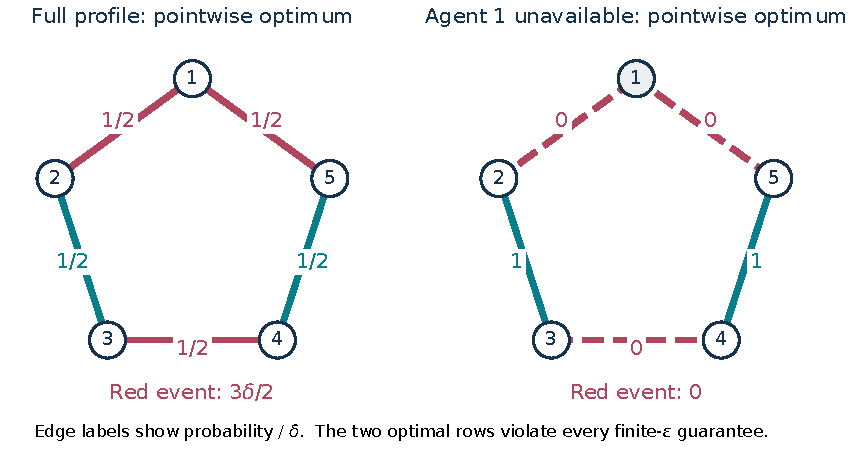
\includegraphics[width=.88\textwidth]{figures/02-obstruction.pdf}
\caption{Incompatible pointwise optima on a five-cycle. Dashed edges have zero output probability. The red event includes two contracts made infeasible by withdrawal and one contract still feasible but assigned zero probability by the new optimizer. Its discrepancy exceeds $\delta$ independently of $\epsilon$.}
\Description{Two five-cycle diagrams compare a uniform half-delta edge distribution to a withdrawal optimum. A red three-edge event has mass three delta over two versus zero.}
\label{fig:obstruction}
\end{figure*}

\subsection{The exact frontier at zero epsilon}
\begin{theorem}[Five-cycle Pareto frontier]\label{thm:frontier}
Among globally feasible $(0,\delta)$-private mechanisms, the nondominated $(h,w)$ pairs are precisely the line segment joining
\begin{equation}\label{eq:endpoints}
 A=(5\delta/2,3\delta/2),\qquad
 B=(25\delta/12,7\delta/4).
\end{equation}
Equivalently, all mechanisms satisfy
\begin{equation}\label{eq:frontier-bounds}
 h\leq5\delta/2,\qquad
 w\leq7\delta/4,\qquad
 w\leq3\delta-3h/5,
\end{equation}
and each point of the stated segment is attainable.
\end{theorem}
\begin{proof}
Average any mechanism over the ten rotations and reflections of the cycle, consistently relabeling inputs and outputs. Feasibility and DP are convex and invariant under these relabelings. The averaging preserves $h$ and $w$. It therefore suffices to bound a symmetric mechanism.

Write its probability per edge at full participation as $a$, so $h=5a$. At a four-agent path, write the three probabilities in path order as $(b,c,b)$, so $w=2b+c$. At a three-agent two-edge path, reflection symmetry gives probabilities $(d,d)$. The central agent's load yields $d\leq\delta/2$.

Delete an endpoint of a four-agent path and consider the event consisting of its two endpoint edges. Its probability is $2b$ before deletion and $d$ afterward. DP gives $2b\leq d+\delta$, hence $b\leq3\delta/4$. The path load constraint $b+c\leq\delta$ then gives $w\leq7\delta/4$.

Next, compare full participation to any four-agent path. The event comprising its two deleted edges and its surviving middle edge has probabilities $3a$ and $c$, respectively. Thus $c\geq3a-\delta$. Since $2(b+c)\leq2\delta$, we obtain $w\leq2\delta-c\leq3\delta-3h/5$. The bound on $h$ follows from Theorem~\ref{thm:row}.

For attainability, mechanism $A$ is the fixed lottery assigning $\delta/2$ to every cycle edge. At a four-agent path it assigns $\delta/2$ to all three feasible edges. Mechanism $B$ is specified on every profile by Table~\ref{tab:mechanisms}; abstention receives the remaining mass. Its largest total mass is $25\delta/12\leq5/6$.

We verify $B$ using total variation. Adding an agent can produce: an empty-to-nonempty transition (total new mass at most $\delta$); a single edge becoming a two-edge path (distance $\delta/2$); a single edge becoming a three-edge path (distance $\delta$); a two-edge path becoming a three-edge path (distance $\delta$); or a three-edge path becoming the full cycle (distance $\delta$). Additions that leave the feasible edge set unchanged leave the row unchanged. These cases exhaust cube edges up to symmetry, so $B$ is $(0,\delta)$-private. Its objectives are exactly the second pair in \eqref{eq:endpoints}.

Publicly randomizing between $A$ and $B$ attains their connecting segment. Every pair with $h<25\delta/12$ is dominated by $B$ or an equally good endpoint; for larger $h$, the final inequality in \eqref{eq:frontier-bounds} is attained on the segment. No pair beyond that segment can be nondominated.
\end{proof}

\begin{table}[t]
\centering
\caption{Contract probabilities divided by $\delta$ in explicit five-cycle mechanisms. Path entries are in edge order. Only feasible edges are listed; the remaining probability is abstention. $A$ assigns $1/2$ to every feasible edge.}
\label{tab:mechanisms}
\begin{tabular}{lcc}
\toprule
Feasible edge structure & $B$: $\epsilon=0$ & $C$: $\epsilon=\log2$\\
\midrule
Empty & --- & ---\\
One edge & $1$ & $1$\\
Two-edge path & $(1/2,1/2)$ & $(1/2,1/2)$\\
Three-edge path & $(3/4,1/4,3/4)$ & $(1,0,1)$\\
Five-cycle & $5/12$ per edge & $1/3$ per edge\\
\bottomrule
\end{tabular}
\end{table}

\subsection{Epsilon changes compatibility, not the row optima}
\begin{proposition}\label{prop:epsilon}
For a public prior uniform over the five profiles with one absent agent, optimal agreement probability is $7\delta/4$ at $\epsilon=0$ and $2\delta$ at $\epsilon=\log2$. Every profile's pointwise optimum remains unchanged.
\end{proposition}
\begin{proof}
The first optimum is Theorem~\ref{thm:frontier}. The second is bounded above by the pointwise value $2\delta$. Mechanism $C$ in Table~\ref{tab:mechanisms} attains this value at every one-withdrawal profile. We check its DP constraints on the full cube using multiplier $e^\epsilon=2$.

Transitions involving only empty sets, single edges and two-edge paths have directed divergences at most $\delta$. Between a single edge and a three-edge path, the larger directed divergence is at most $\max\{\delta,3\delta-1\}=\delta$. Between a two-edge path and a three-edge path, the two divergences are $\delta$ and $\delta/2+[3\delta-1]_+$, both at most $\delta$ for $\delta\leq2/5$. Between a three-edge path and the full cycle, they are $\delta$ and $2\delta/3$: the possible abstention contribution $[7\delta/3-1]_+$ is zero in this range. These exhaust adjacent cases up to symmetry. Normalization and feasibility follow from the table. Theorem~\ref{thm:row} establishes the final assertion.
\end{proof}

The increase is $\delta/4$, or $14.29\%$ relative to the zero-epsilon optimum. It is not a change in the privacy limit of an isolated decision. It arises because the looser multiplicative constraint permits a different collection of rows to coexist. Figure~\ref{fig:frontier} compares the exact zero-epsilon frontier with numerical solutions at larger epsilon.

\begin{figure}[t]
\centering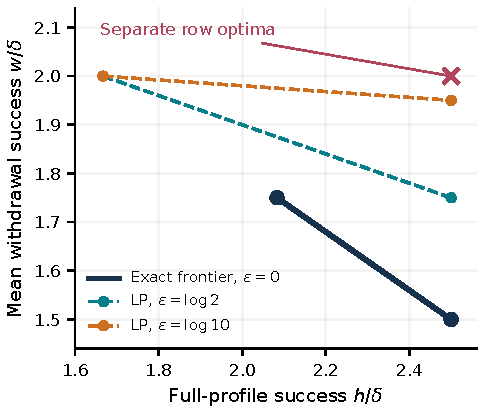
\includegraphics[width=\columnwidth]{figures/03-frontier.pdf}
\caption{Five-cycle compatibility. The solid segment is the exact frontier from Theorem~\ref{thm:frontier}; dashed segments join nondominated full-cube LP solutions at larger epsilon ($\delta=0.1$). The cross combines separately optimal rows and is unattainable for any finite epsilon.}
\Description{Agreement tradeoffs show an exact declining segment at epsilon zero and numerical frontiers at larger epsilon. The combination of pointwise optima is outside every plotted frontier.}
\label{fig:frontier}
\end{figure}

\section{Implementation and Computational Evaluation}\label{sec:experiments}
\subsection{Reference mechanisms and checks}
The packing optimizer uses SciPy 1.13.1's HiGHS interface. A separate full-profile formulation allocates $P_x(o)$ for all $2^n$ profiles and $m+1$ outputs. For every directed cube edge $(x,y)$ and output $o$, it adds $s_{xy,o}\geq0$ satisfying
\[
 s_{xy,o}\geq P_x(o)-e^\epsilon P_y(o),\qquad
 \sum_o s_{xy,o}\leq\delta_i.
\]
Together with row normalization and zero probability for infeasible contracts, these are exactly \eqref{eq:hockey}. The objective is \eqref{eq:bayes}. This is an exponential-state reference oracle, not a scalable implementation claim. It optimizes all rows simultaneously and never restricts the privacy domain to the prior's support.

A separate verifier reads saved distributions and recomputes utilities. It checks all directed cube edges without using the solver's slack variables. On small outputs we additionally enumerate every event. The exhaustive three-agent mechanisms are rationally reconstructed and verified with exact fractions, including both DP and normalization. Rational primal and dual certificates prove each packing optimum by weak duality. Their feasibility and equal objectives are checked with fractions, without trusting solver status. The analytic proofs do not depend on these reconstructions.

The execution prototype accepts rational weights and checks their loads exactly. It draws an integer from a common denominator and applies the feasibility veto. Repeated use of the same object raises an error. This avoids floating-point probability rounding in the sampler. It is a reference implementation: persistent session enforcement, timing protection, distributed trust and production security are not implemented.

\subsection{Declared finite experiments}
The protocol predates the primary runs. It specifies three suites: all nonempty three-agent menus, the cycle tradeoff, and 24 menus generated with fixed seeds for six agents. The later derivation of Theorem~\ref{thm:frontier} and Proposition~\ref{prop:epsilon} was motivated by the cycle results and is documented as exploratory theory.

\paragraph{Exact row characterization.}
There are seven nonempty contracts on three agents and 127 nonempty menus. For each menu we used $\delta\in\{0.01,0.1,0.4\}$ and $\epsilon\in\{0,\log2\}$, with the public-prior objective concentrated on full participation. All 762 full-profile optima matched the packing values within $10^{-7}$. All 381 menu--delta packing instances have rational primal--dual certificates. All 762 saved mechanism distributions passed exact rational DP verification. These results test the implementation against a complete small domain; they do not replace the proof for arbitrary menus.

\paragraph{Cycle and exact arithmetic.}
We solved 63 full-cube LPs: 21 public objective mixtures between full participation and uniform single withdrawal, at each of $\epsilon\in\{0,\log2,\log10\}$ and $\delta=0.1$. For the analytic zero-epsilon segment, a solver-free checker verifies all 64 output events on all 160 directed cube edges for 21 mixtures at each of $\delta\in\{1/100,1/10,2/5\}$. This gives 63 rational mechanisms and 645,120 event inequalities. Three additional rational instances of mechanism $C$ pass 30,720 inequalities at multiplier two. The largest floating-point DP excess in the cycle LP suite was below $2\cdot10^{-16}$.

\begin{table*}[t]
\centering
\caption{Mean expected agreement probability (\%) over 24 synthetic six-agent menus at $\delta=0.1$. Expectations are exact under the declared prior. All methods except the row bound are feasible and private. Fixed policies satisfy $\epsilon=0$ and are therefore unchanged in the $\log2$ rows.}
\label{tab:benchmark}
\begin{tabular}{ccrrrr}
\toprule
$q$ & $\epsilon$ & Uniform & Fixed LP & Adaptive LP & Row bound \\
\midrule
0.5 & $0$ & 3.03 & 5.29 & 7.48 & 7.61 \\
0.5 & $\log 2$ & 3.03 & 5.29 & 7.57 & 7.61 \\
0.8 & $0$ & 9.55 & 14.37 & 16.33 & 16.85 \\
0.8 & $\log 2$ & 9.55 & 14.37 & 16.68 & 16.85 \\
\bottomrule
\end{tabular}

\end{table*}

\begin{figure*}[t]
\centering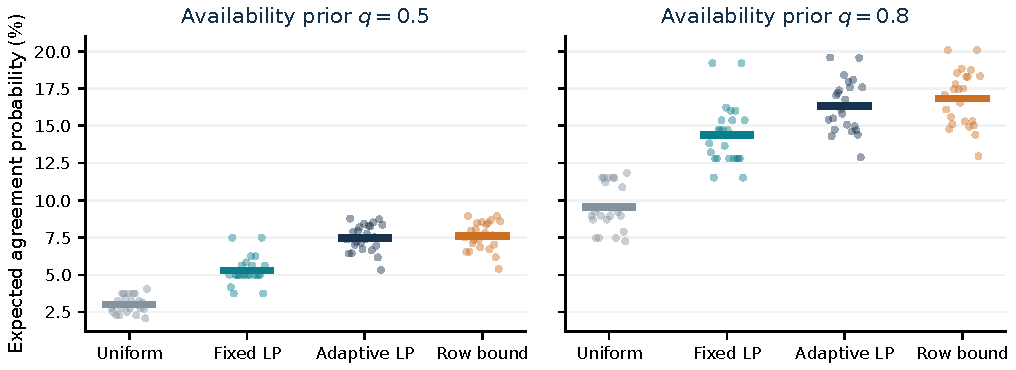
\includegraphics[width=.90\textwidth]{figures/04-benchmark.pdf}
\caption{Menu-level expected agreement rates at $\delta=0.1$, $\epsilon=0$. Each dot is one of the 24 synthetic menus; horizontal marks are means, not confidence intervals. The same menus and priors are used for every method. The row bound allows incompatible, separately optimized mechanisms.}
\Description{Two panels compare uniform, optimized fixed, adaptive, and pointwise-bound agreement rates for 24 synthetic menus at availability probabilities one half and four fifths.}
\label{fig:benchmark}
\end{figure*}

\paragraph{Six-agent policy comparison.}
For each of 24 seeds, we generate a menu of six agents. It has eight distinct contracts, drawn without replacement from all subsets of size two or three. All contracts have unit utility. Each agent is independently available with public probability $q=0.5$ or $q=0.8$. Privacy settings use $\delta\in\{0.02,0.1,0.25\}$ and $\epsilon\in\{0,\log2\}$, giving 288 comparisons. Each expectation sums all 64 input profiles exactly. The uniform fixed lottery uses equal contract mass limited by the largest incidence load. The optimized fixed lottery uses \eqref{eq:prior-lottery}. The adaptive LP is a globally private benchmark; the average pointwise optimum is an upper bound, not an executable policy.

Table~\ref{tab:benchmark} shows the $\delta=0.1$ results. At $\epsilon=0$, adaptive optimization raises mean agreement probability from $5.29\%$ to $7.48\%$ for $q=0.5$, and from $14.37\%$ to $16.33\%$ for $q=0.8$. Increasing epsilon to $\log2$ further raises the adaptive means to $7.57\%$ and $16.68\%$, while the pointwise bounds remain $7.61\%$ and $16.85\%$. Figure~\ref{fig:benchmark} reports the menu-level variation rather than only averages. Results at the other delta values are retained in the artifact; all comparisons used the same fixed menu generator. No deployment distribution or statistical population is inferred from these synthetic menus. The largest floating-point privacy excess across the 288 saved adaptive policies was below $6\cdot10^{-16}$.

\subsection{Negative controls}
Two controls test common implementation errors. First, consider contracts $\{1,2\}$ and $\{1,3\}$ with fixed mass $0.1$ each. At $\epsilon=\log2$, each single-output discrepancy is at most $0.1$, yet their union has discrepancy $0.2$ when agent 1 withdraws. A singleton-only checker falsely accepts a $\delta=0.1$ claim.

Second, renormalizing a valid triangle lottery over feasible contracts makes agreement certain whenever at least one contract is feasible. A neighboring profile can have none, producing divergence one. A feasibility filter that reads private input is not automatically valid post-processing; the one-draw construction requires its own coupling proof. Likewise, independent retries can change an incident-contract event probability from $\delta$ to $1-(1-\delta)^T$. The supplied one-use broker does not silently retry a veto. The test suite contains 22 checks covering these failures, heterogeneous budgets, weighted utilities, boundary profiles, exact sampling and repeated-session rejection.

\section{Implications and Scope}\label{sec:discussion}
\paragraph{A design test for agent brokers.}
The incidence matrix turns a privacy promise into an operational constraint. A broker can inspect the dual certificate before investing in dialogue optimization: if every candidate agreement requires the same protected principal, success cannot exceed that principal's $\delta$. Adding many alternative service providers does not remove this common-party bottleneck. By contrast, disjoint opportunities can increase aggregate success, even though each individual participant remains rarely exposed. The practical output is a bound on what a proposed interface can deliver, together with a reproducible lottery when that bound is useful.

This is a restrictive privacy goal. Public outcome privacy protects the fact of participation itself, whereas a business may only need to hide valuation details conditional on an agreement. Joint privacy, private notifications or a different disclosure contract may be more suitable. Those alternatives change what the observer sees and require their own analysis; they are not consequences of the present theorem. Strong small-delta privacy and frequent named transactions should not be simultaneously advertised under the model studied here.

\paragraph{Where adaptation helps.}
Optimizing a fixed public lottery can waste draws on unavailable contracts. A full-profile mechanism can redistribute probabilities, but only in a way compatible with neighboring inputs. The exact five-cycle result explains why freely re-solving the local LP is invalid, and why a broader privacy budget may improve expected utility without changing any profile's isolated upper bound. It also distinguishes three reporting targets: implementable fixed-policy utility, implementable adaptive utility, and an unattainable average of local optima.

\paragraph{Limits and next questions.}
The model has one bit per agent, a public menu and public utilities, a trusted broker, static inputs and one observable execution. It excludes private menu discovery, multi-attribute acceptability, collusion-resistant distributed implementation, truthful reporting and scheduling multiple contracts. The theory is exact within these assumptions, but the experiments do not establish commercial demand, throughput on a deployed platform, or improved LLM behavior. The generic full-profile optimizer scales exponentially in $n$. Finding tractable menu classes with compatible pointwise optima, and approximating the adaptive optimum without enumerating profiles, are concrete algorithmic questions left open.

\section{Conclusion}
In this model, feasibility bounds how often a given agent can appear in a public agreement. These capacities exactly characterize every attainable row and admit a fixed-lottery extension. They do not characterize which collections of optimal rows can coexist. The five-cycle gives an exact separation, an attainable Pareto frontier, and a strict epsilon-dependent gain in expected success despite epsilon-independent pointwise optima. This distinction supports precise privacy claims and a reproducible audit for agent contracting.

\paragraph{Artifact availability.}
The artifact contains code, saved distributions, exact certificates and figure scripts. It also includes the protocol and supplementary methods. It is available at \url{https://github.com/shi1720/consent-lottery}. All primary calculations are reproducible without model APIs or external datasets.

\balance
\bibliographystyle{ACM-Reference-Format}
\bibliography{references}
\end{document}
